%class
	\documentclass{beamer}

%template
	\usetheme{HannoverSalman}
	\setbeamertemplate{navigation symbols}{}
	%\setbeamertemplate{footline}{\centering{\insertframenumber/\insertpresentationendpage}}
	%\setbeamertemplate{footline}{\hspace*{.5cm}\scriptsize{\hfill\insertframenumber\hspace*{.5cm}}} 


%packages
	\usepackage{amsmath, amssymb, graphicx,cancel}
	\usepackage[absolute,overlay]{textpos}
	\usepackage{subfigure}
	\usepackage{caption}\captionsetup{labelformat=empty,labelsep=none}
	\usepackage{geometry}
	\geometry{verbose}
	\usepackage{color}
	\usepackage{xmpmulti}
	\usepackage[3D]{movie15}
	\usepackage{hyperref}
%	\usepackage{bookmark}
	\usepackage[open,openlevel=4,atend]{bookmark}
	%\bookmarksetup{color=blue}
	\usepackage{multirow}
	\usepackage[style=numeric,defernumbers, authoryear]{biblatex}
	%\usepackage[square,sort]{natbib}
	%\usepackage{fancyhdr}%\pagestyle{fancy} 

	
	\hypersetup{bookmarksdepth = 4}


%citations files
	\bibliography{MyCitations}

%logoCSIPCPL
    \setlength{\TPHorizModule}{1mm}
    \setlength{\TPVertModule}{1mm}
    \newcommand{\logoCSIPCPL}
    {
    	\begin{textblock}{1}(100,2) %(100,85)  for bottom
    		\includegraphics[width=1.5cm]{figs/logo_CSIP}
    	\end{textblock}
    	
	\begin{textblock}{1}(117,1) %(117,85)  for bottom
    		\includegraphics[width=1.0cm]{figs/logo_CPL}
    	\end{textblock} 
    }

%logo evolution
    \newcommand{\logoEvolution}
    {    	
	\begin{textblock}{1}(110,1) %(117,85)  for bottom
    		\includegraphics[width=0.65in]{figs/logo_evolution.pdf}
    	\end{textblock} 
    }

%logo Qualcomm
    \newcommand{\logoQualcomm}
    {
    	\begin{textblock}{1}(110,2) %(100,85)  for bottom
    		\includegraphics[width=1.5cm]{figs/logo_qualcomm.jpg}
    	\end{textblock}
    }
%logo Qualcomm (long)
    \newcommand{\logoQualcommllong}
    {
    	\begin{textblock}{1}(0,0) 
    		\includegraphics[width=1.25in]{figs/logo_qualcomm_long.jpg}
    	\end{textblock}
    }

%logo Tech Tower
    \newcommand{\logoTechTower}
    {
    	\begin{textblock}{1}(0,0) 
    		\includegraphics[width=1.25in]{figs/logo_TechTower.jpg}
    	\end{textblock}
    }

%logo tree
    \newcommand{\logoTree}
    {
    	\begin{textblock}{1}(0,0) 
    		\includegraphics[width=1.25in]{figs/logo_tree.jpg}
    	\end{textblock}
    }
%page numbers
    \newcommand{\mypagenum}
    {
    	\begin{textblock}{1}(1,94) 
		{\tiny \color[rgb]{0.2,0.2,1}\insertframenumber} %\insertframenumber,\insertpresentationendpage, \inserttotalframenumber
    	\end{textblock}
    }
%my footnote citation
	\newcommand{\myFootnoteCitation}[2]
	{
		\footnote{\tiny \citeauthor{#1}, \emph{#2}, \citeyear{#1}.}  %\citeauthor{#1}, \citetitle{#1}, #2 \citeyear{#1}.
	}
%my refer to citation
	\newcommand{\mycite}[1]
	{
		\emph{\citeauthor{#1} (\citeyear{#1})}
	}
%my footnote website citation
	\newcommand{\myFootnoteWebsiteCitation}[1]
	{
		\footnote{\tiny \citeauthor{#1}}
	}

\let\thefootnote\relax\footnotetext{Footnotetext without footnote mark}


%section underline
%\newcommand{\tmpsection}[1]{}
%\let\tmpsection=\section
%\renewcommand{\section}[1]{\tmpsection{\underline{#1}}}



%commands
	\newcommand{\likelihood}{p(Z_k| x_k) }						%likelihood
	\newcommand{\prior}{p(x_k)  } 								%prior
	\newcommand{\posterior} {p(x_k| Z_k)}						%posterior
	\newcommand{\prediction} {p(x_k| Z_{k-1})}					%prediction
	\newcommand{\update} {p(x_k|Z_k)}							%update
	\newcommand{\observations} {p(Z_k)}						%observations
	\newcommand{\prevobservations} {p(Z_{k-1})}				%previous observations
	\newcommand{\dxpk} {dx_{k-1}}							%dx_{k-1}
	\newcommand{\ChapKolm}{\int{p(x_k| x_{k-1})p(x_{k-1}|Z_{k-1})} \dxpk} %Chapman Kolmogorov

	%algorithm specific: JPDAF
	\newcommand{\likelihoodJPDAF}{p(Z_k| \chi, m, Z_{k-1}) }		%1. likelihood
	\newcommand{\priorJPDAF}{p(\chi|m, Z^{k-1}} 				%2. prior	
	\newcommand{\observationsJPDAF} {p(Z_k}					%3. observations
	\newcommand{\posteriorJPDAF} {p(\chi| Z_k)}					%4. posterior

%environments
	\newenvironment{changemargin}[2]
	{
	  	\begin{list}{}
		{
			\setlength{\topsep}{0pt}%
			\setlength{\leftmargin}{#1}%
			\setlength{\rightmargin}{#2}%
			\setlength{\listparindent}{\parindent}%
			\setlength{\itemindent}{\parindent}%
			\setlength{\parsep}{\parskip}%
		}
	  	\item[]
		}
		{\end{list}
	}
%figures

%colors
\definecolor{darkgreen}{rgb}{0,0.5,0}

%personal details
	\author{Salman Aslam}
	\institute{Advisor, Dr Christopher Barnes (ECE)\\Co-advisor, Dr Aaron Bobick (CoC)\\Georgia Institute of Technology}
	\date{}

\begin{document}
%####################################################################################################
\title{Information Theory}
%####################################################################################################
\begin{frame}[plain]\logoTechTower
	\titlepage
\end{frame}

\begin{frame}
\frametitle{Outline}
\logoCSIPCPL\logoTechTower
	\setcounter{tocdepth}{1}	
	\tableofcontents
\end{frame}

%#######################################################################
\section{INTRODUCTION}
%#######################################################################
\begin{frame}
\frametitle{Introduction}
\framesubtitle{Entropy}
\logoCSIPCPL\mypagenum
	\begin{figure}				
		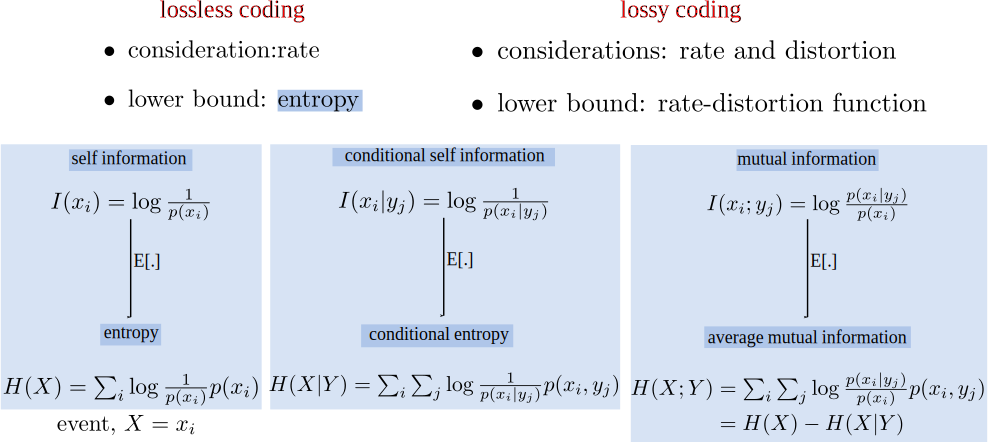
\includegraphics[width=1.0\textwidth]{figs/IT_entropy.pdf}
	\end{figure}
\end{frame}


\begin{frame}
\frametitle{Introduction}
\framesubtitle{Asymptotic Equipartition Property (AEP)}
\logoCSIPCPL\mypagenum
\myFootnoteCitation{1948_JNL_Comm_Shannon}{Bell System Technical Journal}
	\begin{itemize}
		\item AEP is anolog of Law of Large Numbers
		\item we have $n$ i.i.d. random variables, for large $n$
			\begin{equation*}
				\begin{array}{lll}
				\mbox{LLN: }&	\frac{1}{n}\sum\limits_{i=1}^n X_i &\mbox{ is close to } E[X] \\
				\mbox{AEP: }&	\frac{1}{n}\log \frac{1}{p(X_1, X_2, \ldots X_n)} &\mbox{ is close to entropy } H
				\end{array}
			\end{equation*}
	\end{itemize}	
\end{frame}




%=============================================
\subsection{similarity functions}
%=============================================
\begin{frame}
\frametitle{Introduction}
\framesubtitle{Kullback-Leibler (KL) divergence}
\logoCSIPCPL\mypagenum
	\begin{itemize}
		\item {\color {red} author/year}
			\begin{itemize}				
				\item originally introduced by Solomon Kullback and Richard Leibler in 1951
			\end{itemize}
		\item {\color {red} other names}
			\begin{itemize}
				\item information divergence
				\item information gain
				\item relative entropy
			\end{itemize}
		\item {\color {red} category}
			\begin{itemize}
				\item special case of a broader class of divergences called \emph{f}-divergences
			\end{itemize}
		\item {\color {red} attributes}
			\begin{itemize}
				\item {\color {blue} metric}: no (for instance it's not symmetric)
				\item {\color {blue} symmetric}: no
			\end{itemize}
	\end{itemize}	
\end{frame}



\begin{frame}
\frametitle{Introduction}
\framesubtitle{Kullback-Leibler (KL) divergence (cont.)}
\logoCSIPCPL\mypagenum
	\begin{itemize}
		\item average of the logarithmic difference between the probabilities $P$ and $Q$ when the average is taken using the probabilities $P$
			\begin{figure}				
				\includegraphics[width=0.9\textwidth]{figs/IT_KLdivergence.pdf}
			\end{figure}
		where $P$ is the "true" distribution, measure $Q$ typically represents a theory, model, description or approximation of $P$
	\end{itemize}	
\end{frame}



\begin{frame}
\frametitle{Introduction}
\framesubtitle{Bhattacharya coefficient}
\logoCSIPCPL\mypagenum
	\begin{itemize}
		\item {\color {red} attributes}
			\begin{itemize}
				\item {\color {blue} metric}: yes (for instance it's not symmetric)
				\item {\color {blue} symmetric}: yes (since it's a metric)
			\end{itemize}
		\item see \mycite{2003_JNL_TRKkernel_Comaniciu} for details
	\end{itemize}	
\end{frame}


\begin{frame}
\frametitle{Introduction}
\framesubtitle{Packing vs Covering}
\logoCSIPCPL\mypagenum
	\begin{itemize}
		\item Packing: maximize minimum distance
		\item Covering: In the facility location problem, minimize maximum distance that a customer has to travel to new facility{\color{blue}\href{http://en.wikipedia.org/wiki/Smallest_circle_problem}{(wikipedia)}}, also known as \emph{smallest circle problem}
	\end{itemize}	
\end{frame}


%#######################################################################
\printbibliography
\end{document}
%#######################################################################